\chapter{Literature Review and Related Work}
\label{chap:relatedworks}

\section{Competitor Analysis}
\label{section:competitor-analysis}

\begin{figure}[h]
    \centering
    \frame{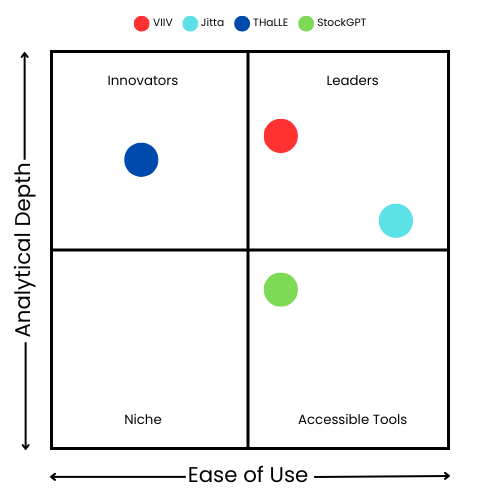
\includegraphics[width=0.7\textwidth]{chapter-2/landscape.png}}
    \caption[Competitive landscape comparison of VIIV, Jitta, THaLLE, and StockGPT]{Competitive landscape comparison of VIIV, Jitta, THaLLE, and StockGPT. Created by the author, accessed 14 March 2025.}
    \label{fig:competitive-landscape}
\end{figure}

Figure \ref{fig:competitive-landscape} illustrates the competitive landscape of VIIV and other stock analysis platforms, evaluated based on Analytical Depth (y-axis) and Ease of Use (x-axis). 
Each competitor is positioned in a quadrant that reflects their strengths and market positioning.

1. \textbf{VIIV (Red, Leaders Quadrant)}

\begin{itemize}[leftmargin=80pt]
    \item VIIV balances both analytical depth and ease of use.
    \item It provides strong analytical capabilities while maintaining an accessible user experience.
    \item VIIV integrates Thai financial data, including 56-1 One Reports, making it an exceptional choice for Thai investors.
\end{itemize}

2. \textbf{Jitta (Light Blue, Leaders Quadrant)}

\begin{itemize}[leftmargin=80pt]
    \item Jitta provides the best ease of use but has a lower level of analytical depth than VIIV and THaLLE.
    \item It offers AI-based stock ratings and valuation tools for value investors.
    \item Jitta’s simplicity makes it user-friendly, but it lacks qualitative insights and real-time market data.
\end{itemize}

3. \textbf{THaLLE (Dark Blue, Innovators Quadrant)}

\begin{itemize}[leftmargin=80pt]
    \item THaLLE focuses on deep analytical capabilities but is only a standalone model.
    \item It is a CFA-trained financial LLM designed for professional-level financial analysis.
    \item THaLLE is not optimized for Thai stocks and does not provide an intuitive interface for general users.
\end{itemize}

4. \textbf{StockGPT (Green, Accessible Tools Quadrant)}

\begin{itemize}[leftmargin=80pt]
    \item StockGPT balances ease of use with AI-driven financial insights.
    \item It specializes in earnings call transcript analysis for US markets (S\&P 500, Nasdaq).
    \item StockGPT lacks Thai stock market coverage, which limits its usability for Thai investors.
\end{itemize}

\newpage

\subsection{Jitta}
\label{subsection:jitta}

\begin{figure}[h]
    \centering
    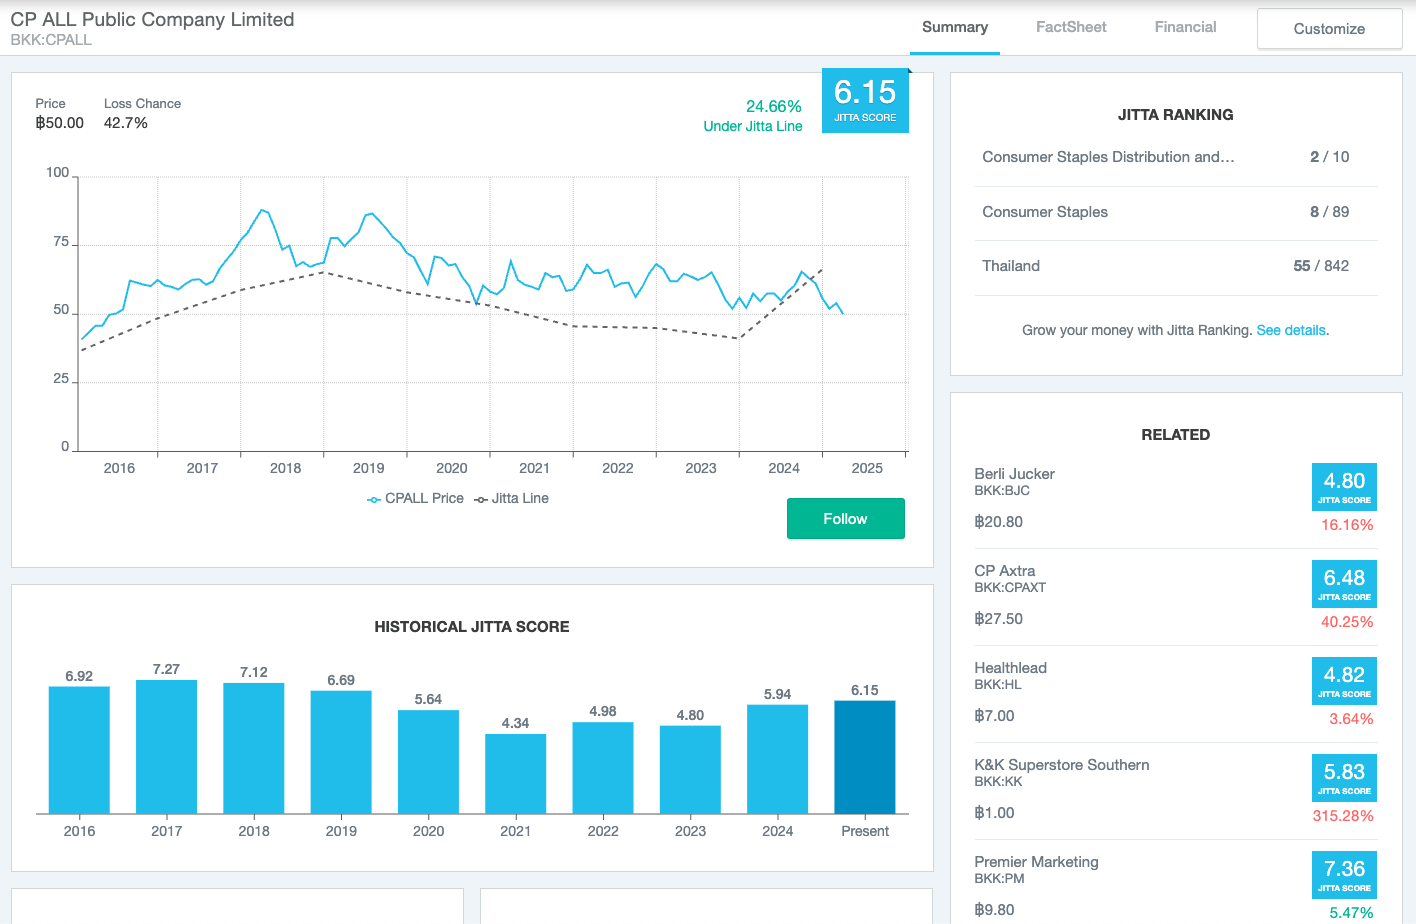
\includegraphics[width=1\textwidth]{chapter-2/jitta.png}
    \caption[Jitta's stock analysis interface for CP ALL]{Jitta's stock analysis interface for CP ALL (BKK:CPALL). Courtesy of Jitta, accessed 14 March 2025, \url{https://www.jitta.com/stock/bkk:cpall}.}
    \label{fig:jitta}
\end{figure}

\FloatBarrier

Jitta is an AI-powered stock rating platform for value investors. It provides fundamental analysis tools to help users make investment decisions. 
The platform evaluates stocks based on quantitative financial data from company statements. This simplifies research by automating complex financial analysis. 
Jitta offers a systematic approach to stock selection. It reduces dependence on subjective judgment.

\begin{itemize}[leftmargin=60pt]
    \item \textbf{Jitta Score}: A stock rating from 0 to 10 based on a company’s financial health and performance. A higher score indicates the company is strong, stable, and consistently profitable.
    \item \textbf{Jitta Line}: An estimated fair value of a stock, calculated using past financial performance. If a stock’s market price is below this line, it may be undervalued and a good buying opportunity.
    \item \textbf{Jitta Ranking}: A ranking system that highlights strong companies with undervalued stock prices. It helps investors find the best opportunities.
    \item \textbf{Stock Analysis}: Jitta covers over 30,000 stocks from 29 countries. It provides a wide range of financial data for global investors.
    \item \textbf{Jitta Wise}: A mobile tool that gives quick, easy-to-understand financial insights about a company. It helps investors make fast decisions.
    \item \textbf{Investment Strategies}: Jitta offers ready-made and customizable filters. These help investors find stocks that match their investment style and goals.
    \item \textbf{Comprehensive Financial Data}: Investors can access 10 years of company financial reports. This helps analyze trends and make informed decisions.
    \item \textbf{Portfolio Management}: Jitta provides tools to track and manage investments. It helps investors optimize their portfolios for long-term success.
\end{itemize}

Jitta focuses mainly on quantitative financial data, allowing investors to assess a company’s financial performance objectively. 
However, it lacks insights from qualitative factors such as management strategy, industry trends, competitive advantages, and macroeconomic influences. 
While Jitta provides a data-driven approach to stock evaluation, investors may still need to work on their research with qualitative assessments to make well-rounded investment decisions\cite{JittaWebsite}.

\newpage

\subsection{THaLLE}
\label{subsection:thalle}

\begin{figure}[h]
    \centering
    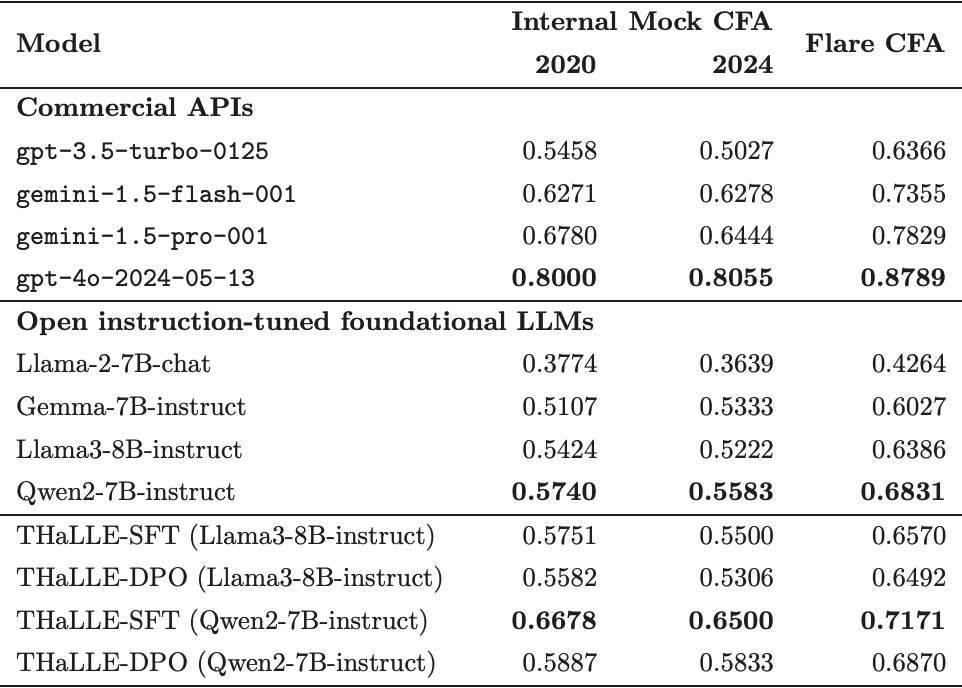
\includegraphics[width=1\textwidth]{chapter-2/thalle.png}
    \caption[THaLLE and other models' performance on CFA exams]{THaLLE and other models' performance on CFA exams. Courtesy of KBTG, accessed 14 March 2025, \url{https://arxiv.org/pdf/2406.07505}.}
    \label{fig:thalle}
\end{figure}

\FloatBarrier

THaLLE (Text Hyperlocally Augmented Large Language Extension) is a financial large language model (LLM) developed by KBTG, specifically trained using Chartered Financial Analyst (CFA) examination data.
It is designed to perform high-level financial reasoning and complex investment analysis at a professional CFA-certified level. By incorporating Supervised Fine-Tuning (SFT) and Direct Preference Optimization (DPO) techniques, 
THaLLE enhances its ability to provide structured financial insights, making it suitable for institutional and professional investors.

\begin{itemize}[leftmargin=60pt]
    \item \textbf{Advanced Financial Reasoning}: Trained on CFA exam materials, THaLLE specializes in complex financial problem-solving, portfolio management, and investment risk assessment.
    \item \textbf{Supervised Fine-Tuning (SFT) and Direct Preference Optimization (DPO)}: Uses these machine learning techniques to enhance its accuracy in financial interpretations and decision-making.
    \item \textbf{AI-Driven Investment Insights}: Capable of analyzing financial concepts such as valuation, risk management, and macroeconomic trends, making it useful for professional financial analysts.
    \item \textbf{Comprehensive Knowledge Base}: Covers global financial theories, investment principles, and professional-level analytical methodologies.
\end{itemize}

While THaLLE represents a significant advancement in financial AI, its focus on professional financial analysis rather than real-time stock evaluation makes it less practical for Thai retail investors.
Its lack of Thai financial data and real-time stock insights creates a gap that VIIV aims to fill by providing a chatbot-driven, Thai-centric stock analysis tool\cite{THaLLEarXiv}.

\newpage

\subsection{StockGPT}
\label{subsection:stockgpt}

\begin{figure}[h]
    \centering
    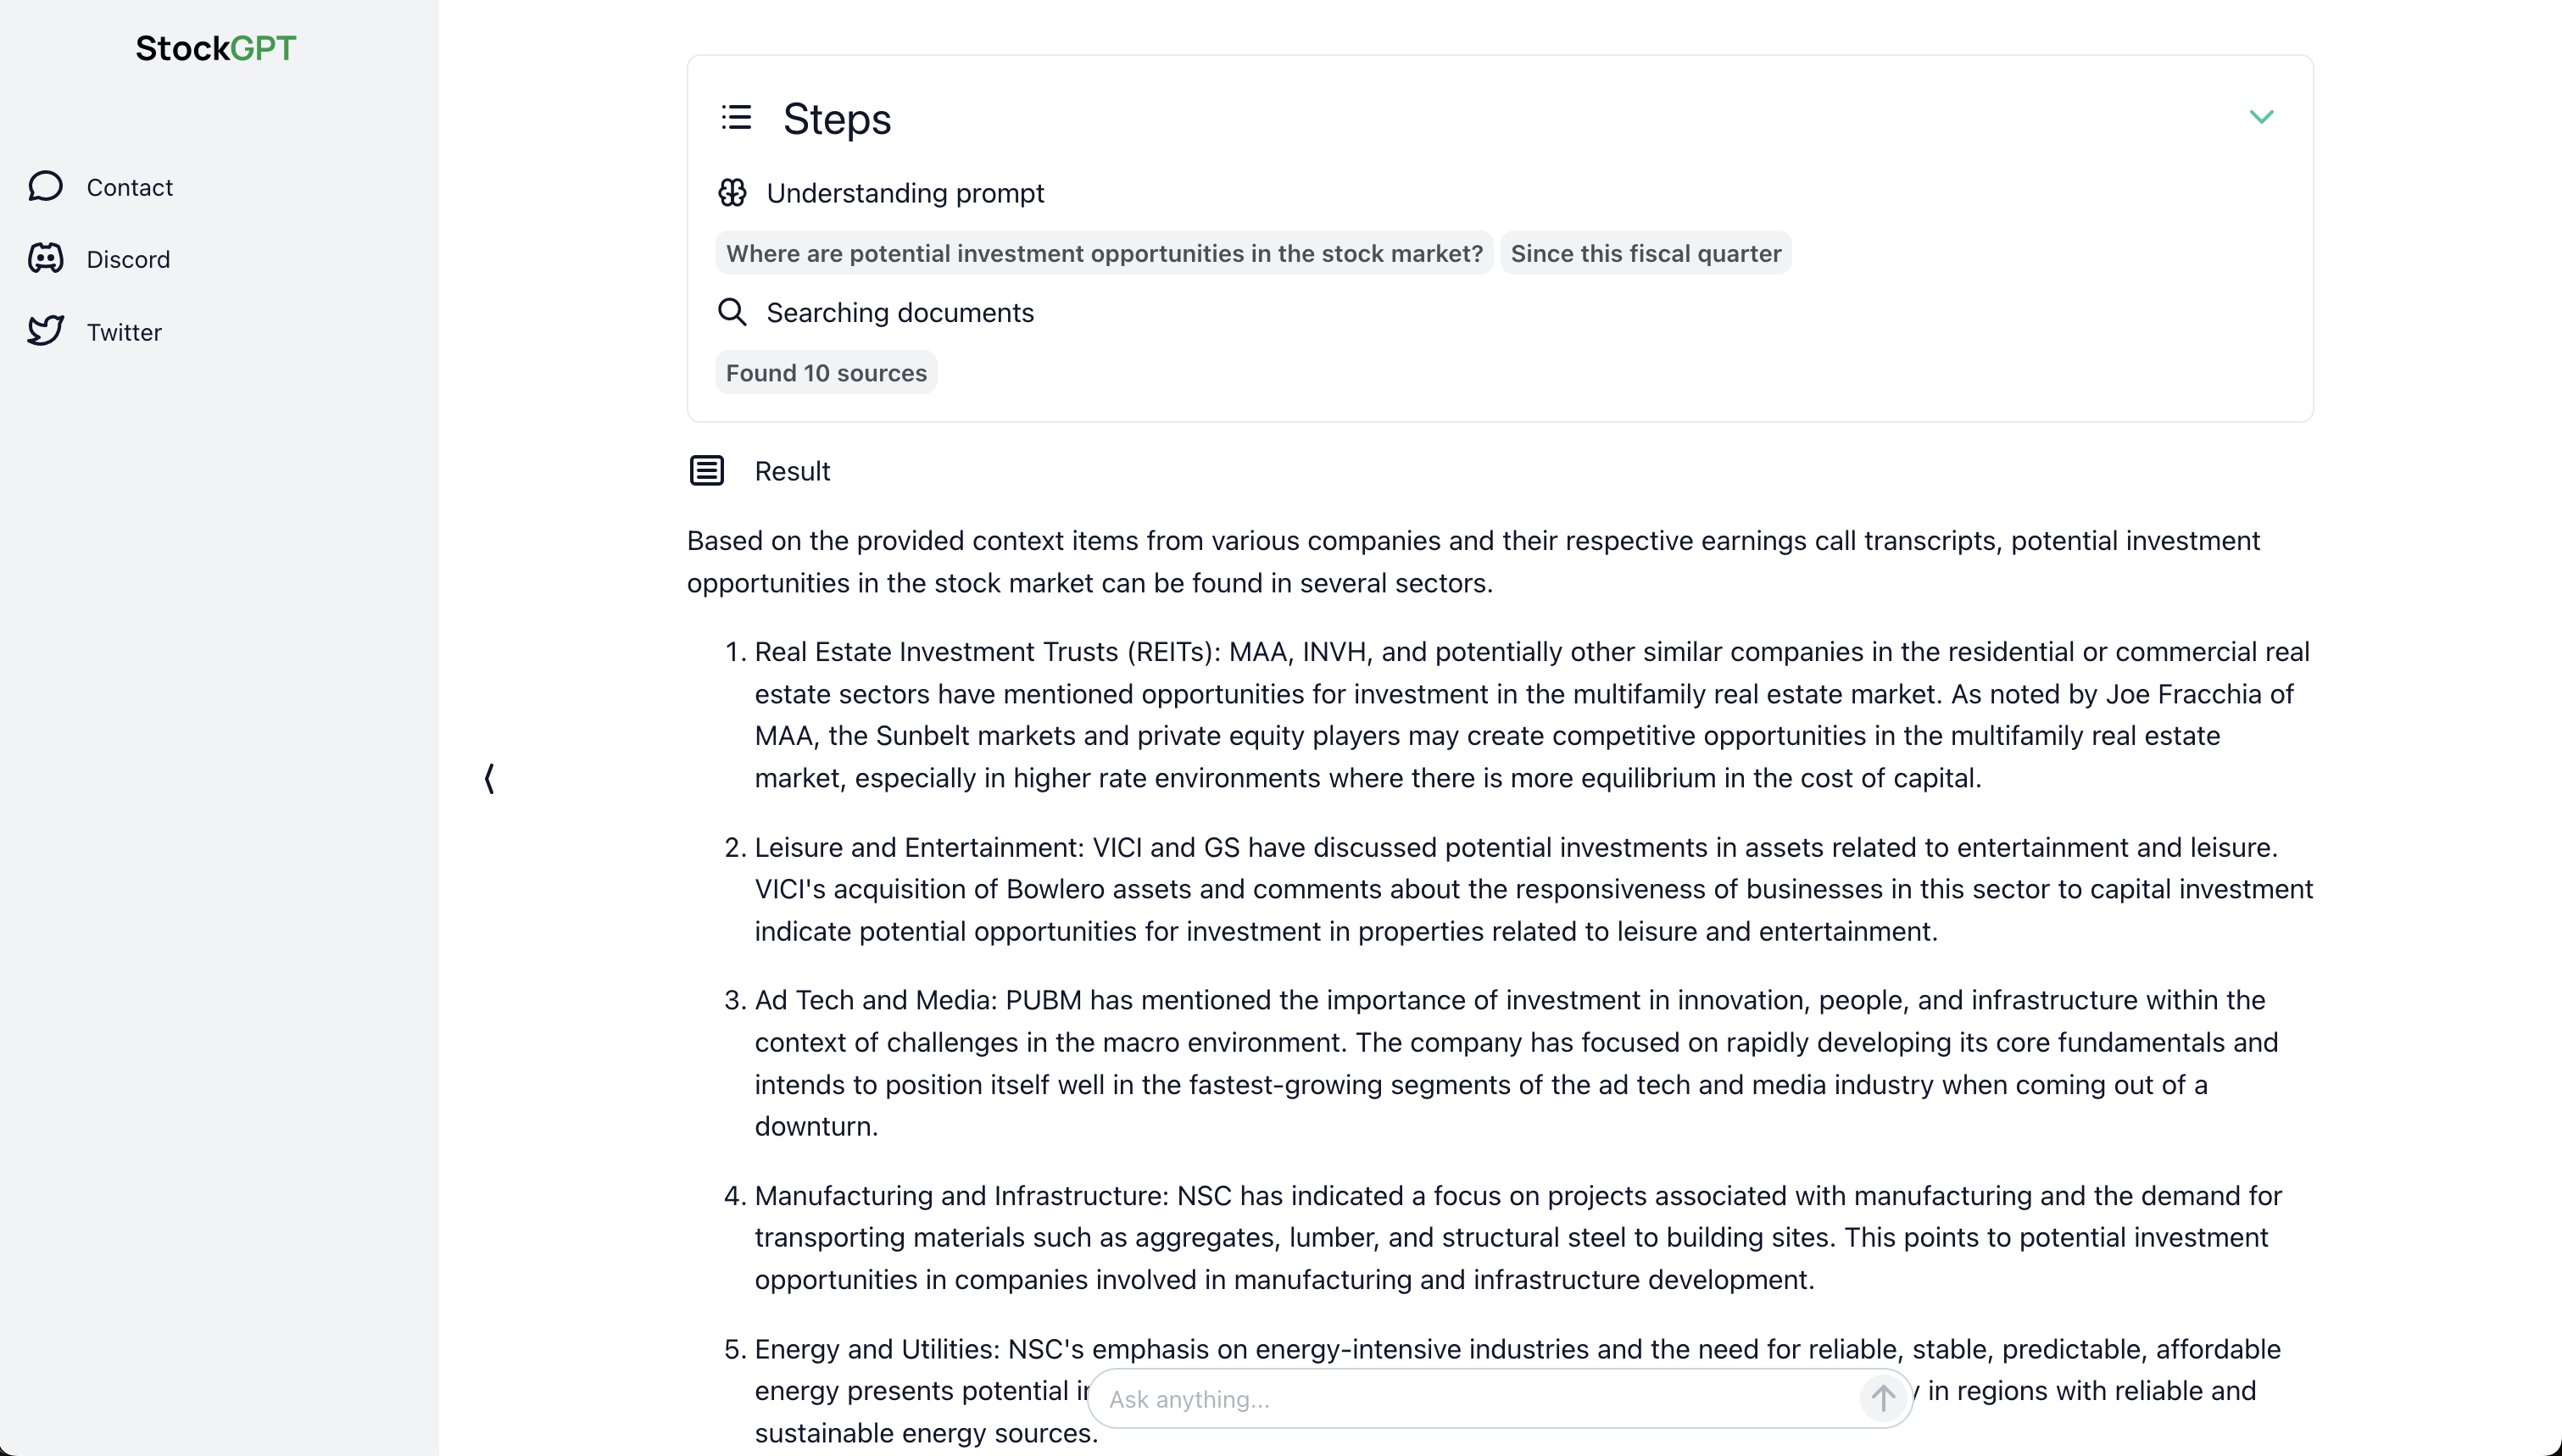
\includegraphics[width=1\textwidth]{chapter-2/stockgpt.png}
    \caption[StockGPT analyzing investment opportunities]{StockGPT analyzing investment opportunities using earnings call transcripts. Courtesy of StockGPT, accessed 14 March 2025, \url{https://askstockgpt.com/}.}
    \label{fig:stockgpt}
\end{figure}

\FloatBarrier

StockGPT is an AI-powered financial research assistant designed for investors analyzing the S\&P 500 and Nasdaq stock markets. 
It specializes in processing and extracting insights from company earnings call transcripts. StockGPT provides up-to-date financial data for informed investment decisions. 
The platform helps investors research company performance, management sentiment, and industry trends efficiently. It reduces the need for manual reviews of lengthy financial 
transcripts by summarizing key points and highlighting relevant insights. The platform's key features include:

\begin{itemize}[leftmargin=60pt]
    \item \textbf{AI-Powered Earnings Call Analysis}: Uses natural language processing (NLP) to analyze company earnings call transcripts, extracting insights related to financial performance and executive sentiment.
    \item \textbf{Timeframe-Based Search}: Allows users to filter earnings call data by specific quarters or years to perform historical performance comparison.
    \item \textbf{Industry and Sector Filtering}: Users can narrow their search to specific industries or sectors to help them focus on relevant companies and trends.
    \item \textbf{Company-Specific Financial Insights}: Retrieves insights on key topics such as revenue growth, market expansion, competitive risks, and cost structures based on what company executives discuss in earnings calls.
    \item \textbf{Customizable Search Queries}: Investors can ask specific questions about companies, trends, or market conditions, receiving AI-generated responses based on factual data from transcripts.
\end{itemize}

Despite its advanced capabilities, StockGPT is limited to analyzing S\&P 500 and Nasdaq stocks. It does not support Thai stock data or integrate with Thai-specific financial reports such as 
the 56-1 One Reports, which are crucial for stock analysis in Thailand\cite{StockGPTWebsite}.

\begin{table}[h]
    \small
    \renewcommand{\arraystretch}{1.5}
    \caption{Comparison of VIIV, Jitta, THaLLE, and StockGPT}
    \label{tab:comparison}
    \begin{tabularx}{\textwidth}{|
        >{\raggedright\columncolor{gray!30}}X |
        >{\raggedright\arraybackslash}X|
        >{\raggedright\arraybackslash}X|
        >{\raggedright\arraybackslash}X|
        >{\raggedright\arraybackslash}X|}
        \hline
        \rowcolor{gray!30} \textbf{Feature} & \textbf{VIIV} & \textbf{Jitta} & \textbf{THaLLE} & \textbf{StockGPT} \\
        \hline
        \textbf{Primary Users} & Thai retail \& professional investors & Value investors (Thai \& global) & Thai finance professionals & US stock investors \\
        \hline
        \textbf{Stock Coverage} & \cellcolor{yellow!30}SET (Stock Exchange of Thailand) & \cellcolor{yellow!30}Thai \& global stocks & \cellcolor{yellow!30}Not stock-specific & \cellcolor{yellow!30}S\&P 500, Nasdaq \\
        \hline
        \textbf{AI Capabilities} & \cellcolor{yellow!30}LLM-powered chatbot for Thai stocks & \cellcolor{yellow!30}AI-based stock ratings \& valuation & \cellcolor{yellow!30}CFA-trained LLM for finance & \cellcolor{yellow!30}AI-driven analysis of earnings calls \\
        \hline
        \textbf{Financial Reports} & \cellcolor{yellow!30}Analyzes Thai 56-1 One Reports \& financial statements & \cellcolor{yellow!30}Extracts data from company filings for ratings & \cellcolor{yellow!30}Can analyze financial concepts, but lacks stock-specific insights & \cellcolor{yellow!30}Focuses on US earnings transcripts \\
        \hline
        \textbf{Sentiment Analysis} & Uses IAA Consensus Sentiment & No sentiment analysis & No sentiment analysis & Analyzes sentiment from earnings calls \\
        \hline
        \textbf{Technical Analysis} & Uses Trend-based Indicators & No technical analysis features & No technical analysis features & No technical analysis features \\
        \hline
        \textbf{Language Support} & \cellcolor{yellow!30}Fully supports Thai & \cellcolor{yellow!30}Thai \& English & \cellcolor{yellow!30}Limited Thai proficiency & \cellcolor{yellow!30}English-only \\
        \hline
        \textbf{Market Data Updates} & \cellcolor{yellow!30}Real-time Thai stock market data & \cellcolor{yellow!30}Updates 2 days after financial filings & \cellcolor{yellow!30}No real-time market data & \cellcolor{yellow!30}Live financial updates for US stocks \\
        \hline
        \textbf{User Interface} & Web-based chatbot assistant & Web/mobile-based stock analysis platform & Model-only, lacks user interface & Chatbot-style interface \\
        \hline
        \textbf{Accessibility} & Open to Thai investors of all levels & Free basic features, paid premium tools & No public access yet & Free \& paid plans, public access \\
        \hline
    \end{tabularx}
\end{table}